%\subsection{\rccl Architecture}\label{sec:design}



%% Describe architecture of the tool.  How we parse IOS/JunOS into an
%% intermediate format.  Describe the intermediate format, how we organize
%% checks in terms of mysql queries, etc. Three phases: 1. preparsing,
%% 2. parsing, 3. checking


%This section describes the high-level architecture of \rccns.  We
%present the design of \rccns's {\em intermediate configuration format},
%a vendor-independent representation of a network's BGP configuration.
%We then briefly describe the correctness tests that \rcc performs,
%noting how the intermediate configuration format facilitates many of
%these tests.



%\subsection{Verifying the Configuration}


%The intermediate format concisely represents configuration semantics and
%allows an operator to see the entire configuration at a glance.  The
%format implicitly specifies a model of network-wide routing
%configuration.  

%% We decided that the intermediate format should not make
%% any assumptions about how the network structure; rather, the
%% intermediate format should be a general, literal interpretation of the
%% configuration, and the queries against the intermediate format should
%% determine the semantics of the intermediate format.
%% %Accordingly, we had to decide
%% %whether the intermediate format should incorporate strict assumptions
%% %about the network configuration, or whether the format should be general
%% %enough to accept configurations that might not necessarily conform to
%% %the data model:
%% %
%% %\begin{itemize}
%% %\itemsep=-1pt
%% %\item What assumptions about network structure should be built into the
%% %intermediate format?  Should the format impose constraints on the
%% %configuration? 
%% %\end{itemize}
%% On one hand, incorporating strict assumptions about network structure
%% makes certain types of verification tests easier because the
%% intermediate format is guaranteed to conform to the strict model.
%% However, it also means that unorthodox configurations may not conform to
%% the model.  Adopting a more general structure allows unusual
%% configurations to be represented in the intermediate format, but it can
%% verification more difficult because the semantics of the intermediate
%% format are less explicit.

%% For example, the table of BGP sessions contains a column for a
%% ``remote AS''.  A remote AS is typically a unique number and represents a
%% distinct administrative domain, but, in certain cases,
%% the same remote AS may actually connect to {\em different} neighboring
%% networks: an ISP may assign the same AS number to multiple customers if
%% those customers have no other upstream providers.  
%% %In this case, the ISP
%% %should remove the ``customer'' AS number from the AS path before
%% %re-advertising the route.  
%% A single administrative domain
%% may also comprise multiple ASes~\cite{rfc-confederations}.

%% A strict data model might impose a one-to-one mapping between an AS and
%% an administrative domain, which would make certain
%% correctness tests easier: \rcc would know that all private AS numbers
%% should be removed on sessions to remote ASes, and, when comparing
%% policies across multiple sessions to the same AS number, it could know
%% that those policies were being applied to the same neighboring network.  
%% A more general data model would accept the configuration information,
%% even if the configuration was not sensible, and rely on the
%% verification process to report possible problems.  This approach
%% may cause the verifier to generate false positives: for example, the
%% verifier may wrongly report that a private AS should be removed from the
%% AS path of an ``eBGP'' session, when, in fact, the ``eBGP'' session is
%% a session to a router with a different AS number in the same
%% administrative domain.

%% Because BGP configuration is flexible, it is difficult to design a
%% strict format that will accept all sensible
%% configurations.  (In Section~\ref{sec:evaluation}, we will describe many
%% anomalies that \rcc discovered that illustrate that BGP can be
%% configured in many different ways to achieve the same task.)  We decided
%% that the
%% intermediate format should serve as a literal representation of the
%% configuration, without applying any sanity checks.  This decision has
%% worked well in practice: the fact that \rcc can load any configuration
%% into the intermediate format (rather than rejecting a configuration
%% because it does not fit the data model) allows it to be considerably
%% more usable.  Although this approach generates more false positives,
%% distinguishing more serious errors from ``anomalies'' has proved to be
%% relatively easy in practice.


%\subsection{Checking the Constraints}
%\label{s:verification}


\subsection{Completeness and Soundness}


\begin{figure}[t]
\centering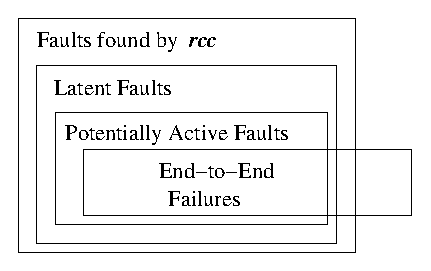
\epsfig{file=rcc/figures/faults2.eps, width=0.6\linewidth}
\caption{Relationships between faults and failures.}
\label{fig:faults}
\end{figure}

%% caveats and setting the fence
%\rccns's constraints are neither complete (\ie,
%they may not find all problematic configurations) nor sound (\ie, they
%may report problems that are simply deviations from best common
%practice), but static analysis techniques for program analysis
%are typically neither complete nor sound either~\cite{Musuvathi2003}.
%As discussed in Section~\ref{sec:mapping}, \rcc is neither complete nor
%sound.  
\rccns's constraints are neither complete nor sound; that is, they may
not find all problematic configurations, and they may complain about
harmless deviations from best common practice.  However, practical
static analysis techniques for program analysis are typically neither
complete nor sound, either~\cite{Musuvathi2003}.
Figure~\ref{fig:faults} shows the relationships between classes
of configuration faults and the class of faults that \rcc detects.  {\em
Latent faults} are faults that are not actively causing any problems but
nonetheless violate the correctness constraints.  A subset of latent
faults are {\em potentially active} faults, for which there is at least
one input sequence that is certain to trigger the fault.  For example,
an import policy that references an undefined filter on a BGP session to
a neighboring AS is a potentially active fault, which will be triggered
when that neighboring AS advertises a route that ought to have been
filtered.  When deployed, a potentially active fault will become {\em
active} if the corresponding input sequence occurs.  An active fault
constitutes a routing failure for that AS.

Some active faults may ultimately appear as {\em end-to-end failures}.
For example, if an AS advertises an invalid route (\eg, a route for a
prefix that it does not own) to a neighboring AS whose import policy
references an undefined filter, then some end hosts may not be able to
reach destinations within that prefix.  Note that a 
potentially active fault may not always result in an end-to-end failure
if no path between the sources and destinations traverses the routers in
the faulty AS.  

\rcc detects a subset of latent (and hence,
potentially active) faults.  In addition, \rcc
may also report some false positives: faults that violate the
constraints but are {\em benign} (\ie, the violations 
would never cause a failure).
Ideally, \rcc would detect fewer benign faults 
by testing the BGP configuration against an abstract specification.
Unfortunately,
producing such a specification requires additional work from
operators, and operators may well write incorrect specifications.  
One of \rccns's advantages is that it provides useful information about
configuration faults without requiring any additional work on the part
of operators.


Our previous work~\cite{Feamster2003b} presented three properties in
addition to path visibility and route validity: information flow control
(this property checks if routes ``leak'' in violation of policy),
determinism (whether a router's preference for routes depends on the
presence or absence of other routes), and safety (whether the protocol
converges)~\cite{Griffin2002c}.  Our definitions of route validity
(Definition~\ref{defn:rv}),
policy (Definition~\ref{defn:policy}), and policy-conformant paths
(Definition~\ref{defn:pcp}) incorporate the notion of information flow
control.  With a couple of exceptions (see Table~\ref{tab:rcc_tests}),
\rcc does not check for faults related
to determinism and safety.  Many aspects of determinism depend on the
route selection process that are inherent in today's practices (\eg, the
fact that MED is only comparable across routes received from the same
neighboring AS) and cannot be effectively checked using static analysis.
Safety is a property of the global routing system that, in practice,
requires access to configurations from multiple ASes to check.  In
Chapter~\ref{chap:policy}, we derive constraints that guarantee safety
with access to configurations of only a single AS and find that these
conditions are quite restrictive.


%\subsubsection{Intermediate Format Overview}








%%%%%%%%%%%%%%%%%%%%%%%%%%%%%%%%%%%%%%%%%%%%%%%%%%%%%%%%%%%%%%%%%%%%%%
%Since the intermediate format is simply a set of relational
%database tables, \rcc can check each correctness constraint by
%executing one ore more SQL queries against the database containing the
%configuration state.


%\footnote{We implemented all
%  correctness checks from 
%Section~\ref{sec:analysis} except those from previous
%work~\cite{Griffin2002}, which require knowledge about shortest
%IGP paths through the network, but, due to space constraints, we
%describe only two checks here: one ``single router'' check, and one that
%requires testing properties of the graph.}  

%Certain 
%queries involve comparing the entries from two tables. For example,
%\rcc checks whether every route that is originated by BGP has a
%corresponding route; this requires comparing entries in the {\tf
%networks} table against those from the {\tf routes} table.


%However, \rccns's extensible design
%facilitates adding these checks.

%% (might allude here to simple checks vs. complex checks)  not really
%% going to discuss pattern-based vs. whatever anymore.  simple checks
%% reall just entail checking bit-flips.  complex can involve multiple
%% routers, interaction with IGP, etc.

%% Also discuss the need to know default settings sometimes.  That is, even
%% the simple ``bit flip'' checks have subtleties.  For example, the avici
%% (and procket) story, where ``no sync'' is enabled by default.  An ideal
%% version of the checker should keep track of routing vendor, OS version
%% numbers, etc., and a detailed list of what's enabled/disabled by default
%% for a particular router.



%%\subsection{\rccl Intermediate Configuration Format}\label{sec:if}





